% The specimen group's own manuscript. It is small on purpose: its job is to
% COMPILE, so that the section shape, the display shape and the generated
% bibliography are proven to reach a reader rather than asserted to.
%
%   cd _fixture && pdflatex QBt-page-types && bibtex QBt-page-types \
%                  && pdflatex QBt-page-types && pdflatex QBt-page-types
%
% `article` rather than misqdoc.cls: this fixture is not a MISQ submission and
% a class it does not need would be cargo. `misq.bst` IS used, because the
% venue type is a MIRROR and its artifact has to do real work here or the
% mirror is decoration.
\documentclass[11pt]{article}
\usepackage[margin=1in]{geometry}
\usepackage{graphicx}
\usepackage{booktabs}
\usepackage{caption}
\usepackage{natbib}
\usepackage[hidelinks]{hyperref}
\title{QBt: a worked example of every board page type}
\author{Specimen group, boardform board}
\date{}
\begin{document}
\maketitle

\begin{abstract}
This document exists to be built, not to be read for its findings. It is the
manuscript half of \texttt{QBt-page-types/}, the specimen group that carries one
worked page per board page type. Everything here is produced by the same tools
the live papers run: the figure by its own recipe, the shipped display folder by
\texttt{build-displays.py}, the bibliography by \texttt{bib-from-bank.py} from a
shared bank. If any of those is broken, this document fails to compile, which is
the only property it is trying to have.
\end{abstract}

\section{What a page type owns on disk}
\label{sec:page-types}

A board page type has always been described by what a page \emph{is}: how it
resolves, how it closes, which typed records it fills. That description is
complete for reading a page and incomplete for building one, because a page of
some types also owns files. Ten contracts govern the types today and between
them they name six artifact paths, so a writer opening a display page for the
first time learns what the page must argue and not what folders it must create.

Five shapes cover the ten types. A \textsc{unit} type owns a folder on both
sides, an authoring folder that is worked in and a shipped folder that is
generated from it; display and slide are its two members. A \textsc{section}
type owns one flat file at the paper root and never a subdirectory of its own.
A \textsc{qa-probe} type owns a folder of evidence records named for the page
that asked; literature and value are its two members, and literature also emits
a bibliography generated from a shared bank. A \textsc{mirror} type owns nothing
and annotates a folder someone else already maintains: venue points at a shared
venue playbook, design at the candidate folder its downstream display unit keeps,
and skill at the skill folder it mirrors. A \textsc{none} type owns nothing at
all, which is the honest answer for stage and meeting.

The shapes are not symmetric in who may act on them, and the display unit shows
this most sharply. Figure~\ref{fig:display-pipeline} draws the eleven steps that
produce one unit. Two of the eleven may be taken by a script, and both are
mechanical: compiling the standalone preview, and copying the selected artifact
into the shipped tree. The rest are a person's, and the three steps of the
acceptance lane are a person's without exception. A machine may render a display
and may ship it. No machine may accept one, because acceptance is of a specific
render rather than of a name, and only a reader can say that the thing in front
of them carries the claim it was asked to carry.

%% GENERATED by board/haipipe-board/cli/build-displays.py from
%%   ../display/QBt3-for-display/float.tex
%% Do not edit this file. Edit the copy under ../display/ and rebuild.
\begin{figure}[t]
  \centering
  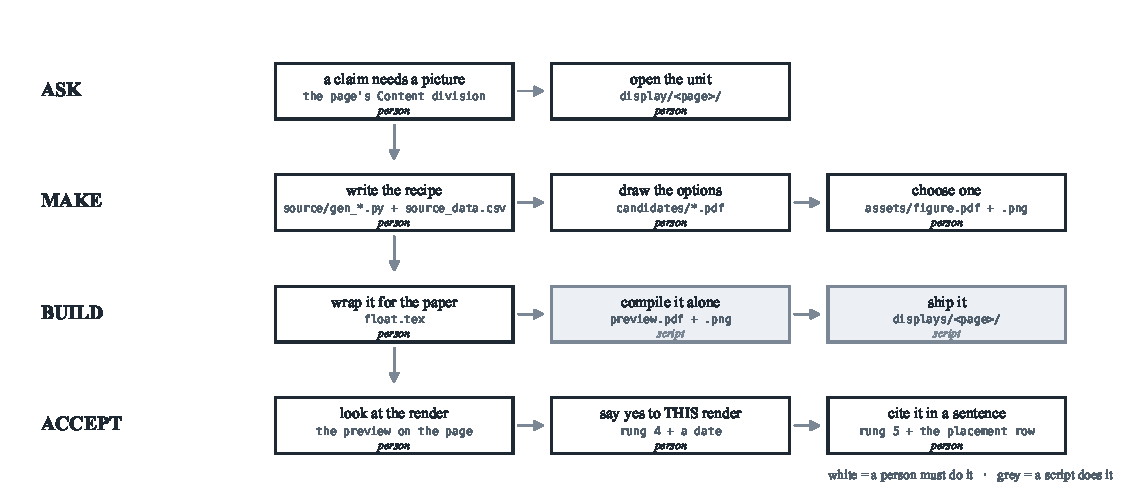
\includegraphics[width=0.95\textwidth]{displays/QBt3-for-display/assets/figure.pdf}
  \caption{How one display unit is produced, and who is allowed to do each step.
  Four lanes, eleven steps, read left to right within a lane and top to bottom
  between them. A white box is a step a person must take; a grey box is a step a
  script takes. Only two of the eleven are grey, and both sit in BUILD: the
  standalone preview compile, and the copy into \texttt{displays/}. Every step in
  ACCEPT is white, which is the rule this figure exists to make visible: a
  machine may render a display and may ship it, and no machine may accept one.
  Drawn from \texttt{source/source\_data.csv} at build time; the lane order is
  the only thing the plotting code hardcodes.}
  \label{fig:display-pipeline}
\end{figure}


The practical consequence is that a contract stated in prose cannot fail, and a
specimen can. A prose contract that never mentions \texttt{float.tex} reads
exactly as well as one that does; a specimen folder missing \texttt{float.tex}
does not build. That asymmetry is the argument for keeping a worked example of
every type on disk and running the real tooling against it, rather than
describing each type and trusting the description.

\section{Measuring with a language model}
\label{sec:llm-measurement}

This section exists so the literature specimen has somewhere to land. Every key
below is claimed on \texttt{QBt4-for-literature.md} and resolves in the shared
bank, and the sentences say only what those sources actually say.

Large language models acquired their general few-shot behaviour at scale, which
is what made them usable as measurement instruments without task-specific
training \citep{brown2020language}. Applied to personality specifically, a
language model has been used to augment text before a smaller model performs
the detection, rather than being trusted to produce the label alone
\citep{hu2024llm}. Surveys of medical applications catalogue the same
opportunity alongside the same reservations about reliability and evaluation
\citep{Nazi2024LLMHealthcare}. None of this settles whether an online rating is
a valid signal about a physician in the first place, which is a separate
question with its own evidence: patient ratings have been compared directly
against physician peer review \citep{mcgrath2018validity}.

The point for a page-type specimen is mechanical rather than substantive. Each
of the four keys was CLAIMED on a literature page with a sentence saying what
job the source does, and each is cited here. The bibliography this document
prints was generated from those two facts and from nothing else: no key was
copied into a local file by hand, and a key that no page claims and no section
cites does not appear.


\bibliographystyle{misq}
\bibliography{QBt-page-types}
\end{document}
